\documentclass[12pt, letterpaper]{book}
\usepackage{graphicx} %LaTeX package to import graphics
\graphicspath{{../Immagini}} %configuring the graphicx package
\usepackage[T1]{fontenc}
\usepackage[italian]{babel}
\usepackage{hyphenat}
\hyphenation{mate-mati-ca recu-perare}
\usepackage{array}
\usepackage{booktabs} % Per linee orizzontali migliori
\usepackage{siunitx}  % Per formattare le unità di misura
\usepackage{caption}  % Per personalizzare le didascalie
\usepackage{multirow} % Per combinare celle nelle colonne
\usepackage{float}
\usepackage{hyperref}

%Domande:
%1) nei dispositivi che stiamo studiando il body è cortocircuitato con il source? 

% grafici che rappresentano l'andamaneto delle Vth al variare di W e L con i tre metodi 
% 

\begin{document}



\chapter{Estrazione dei parametri statici}

\section{Tensione di soglia}

La tensione di soglia $V_{th}$ di un transistore MOS è definita come quella tensione tra gate e bulk per la quale la popolazione di minoritari all'interfaccia è uguale alla popolazione di maggioritari nel bulk. Questa definizione non può essere usata direttamente per il calcolo della tensione di soglia dei dispositivi, ma si deve passare attraverso l'analisi delle caratteristiche corrente-tensione dei dispositivi. \\
Per l'estrazione del parametro $V_{th}$ esistono numerosi metodi, ognuno con punti di forza e punti di debolezza diversi. La scelta di quale metodo utilizzare non è banale e per farla occorre analizzare le caratteristiche di ciascun metodo e confrontare i risultati che offrono. Per questo studio sono stati presi in considerazione:

\begin{itemize}
  \item \emph{Transconductance Change Method (TCM)};
  \item \emph{Second Difference of the Logarithm of the drain current Minimum method (SDLM)};
  \item \emph{Extrapolation in the Linear Region method (ELR)}.
\end{itemize}


\subsection{Transconductance Change Method}

Il \emph{Transconductance Change Method, TCM,} defiscisce la tensione di soglia come la tensione di gate $V_{GS}$ corrispondente al picco massimo della derivata della transconduttanza $g_m$ rispetto alla tensione di gate ($\frac{dg_m}{dV_ {GS}}$) ed è valido per bassi valori della tensione $V_{DS}$.\\
Questa definizione si basa sul fatto che, quando il dispositivo passa dalla regione di debole inversione alla regione di forte inversione, la dipendenza della corrente di drain ripetto a $V_{GS}$ passa dall'essere esponenziale all'essere quasi constante.
La transconduttanza è definita come la derivata prima della corrente $I_D$ rispetto alla tensione $V_{GS}$, dunque la derivata della $g_m$ corrisponde alla derivata seconda di $I_D$. Per questo motivo, il massimo di $\frac{dg_m}{dV_{GS}}$ coincide con la tensione alla quale il grafico della corrente passa dalla forma esponenziale a quella quasi constante, ovvero la tensione $V_{GS}+V_{DS}$. Se $V_{DS}$ è piccola, la tensione per la quale la $g_m$ è massima è molto simile a $V_{th}$.\\

\begin{figure}[h!]
  \centering
  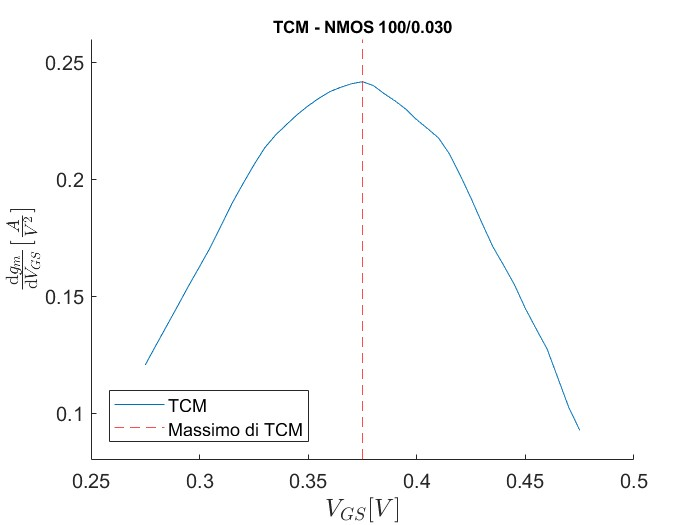
\includegraphics[width=0.49\textwidth]{TCM-N4-100-30-NoFit}
  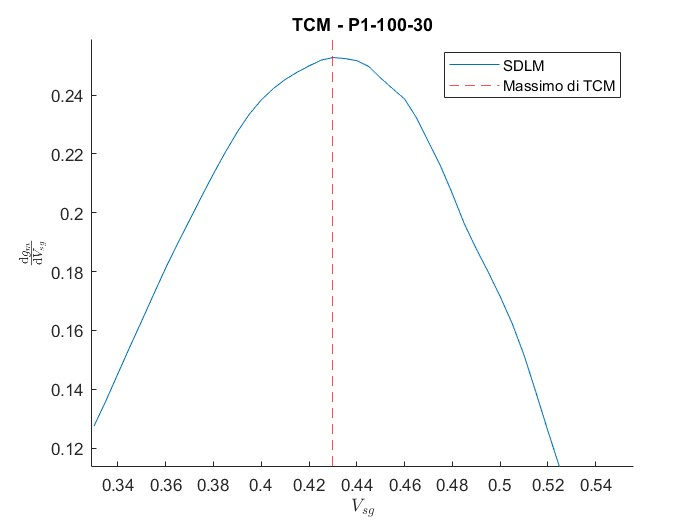
\includegraphics[width=0.49\textwidth]{TCM-P1-100-30-NoFit}
  \caption{Esempio di \emph{TCM} usato su un dispositivo NMOS e un dispositivo PMOS di dimensioni 100-30 a $V_{DS} = 150 mV$}
\end{figure}

\emph{TCM}, poiché si basa sul massimo di una funzione, è molto sensibile ai picchi dovuti ad errori di misura e perciò non è molto affidabile: è quindi necessario rendere la funzione studiata meno dipendente dai campionamenti fuori scala. Inoltre, la risoluzione del dispositivo di misura utilizzato e di $5 mV$, il che rende i valori ottenuti della $V_{th}$ molto approssimativi.
Per far fronte a questi due problemi, si è scelto di non tenere conto del massimo direttamente ottenuto dallo studio di $\frac{dg_m}{dV_{GS}}$ ottenuto dai valori delle misure, ma di interpolare prima i punti del grafico con una funzione polinomiale e, solo a questo punto, di prendere in considerazione il picco di massimo. \\

\begin{figure}[H]
  \centering
  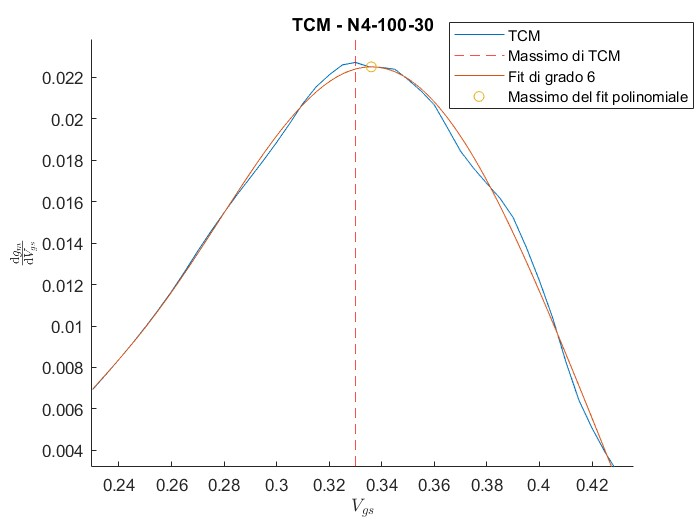
\includegraphics[width=0.49\textwidth]{TCM-N4-100-30}
  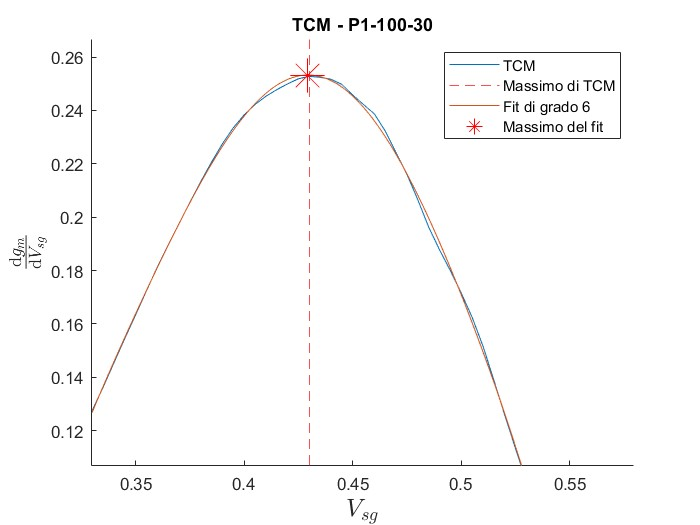
\includegraphics[width=0.49\textwidth]{TCM-P1-100-30}
  \caption{Esempio di \emph{TCM} con fit polinomiale usato su un dispositivo NMOS e un dispositivo PMOS di dimensioni 100-30 a $V_{DS} = 150 mV$}
\end{figure}

Lo studio del fit polinomiale risolve il problema della bassa risolizione di misura e il problema della presenza di valori fuori scala, ma presenta una potenziale nuovo problema: il valore della $V_{th}$ calcolata potrebbe variare significativamente al variare del grado della funzione polinomiale interpolante.
Prendendo come esempio i dispositivi PMOS, si è studiato quanto cambia il valore della tenzione di soglia al variare del grado del fit polinomiale, prendendo in considerazione i gradi di valore 2, 4, 6 e 8, tabella \ref{tab:GradiTCM}.\\

\begin{table}[h]
  \renewcommand{\arraystretch}{1.3}
  \centering
  \begin{tabular}{m{2cm} m{2cm} m{2cm} m{2cm} m{2cm}}
    \toprule
    \multirow{2}{*}{Dispositivo} & \multicolumn{4}{c}{$V_{th} [mV] \text{ con grado:}$} \\
    \cmidrule{2-5}
                                  & 2 &4 &  6 & 8 \\
    \midrule
    100 - 30                     & 426.9   & 429.4   & 429.4   & 430.8   \\
    \hline
    100 - 60                     & 467.6   & 469.5   & 469.3   & 468.9   \\
    \hline
    200 - 30                     & 495.6   & 495.6   & 495.3   & 495.5   \\
    \hline
    200 - 60                     & 397.8   & 399.7   & 399.3   & 399.8   \\
    \hline
    200 - 180                    & 452.2   & 454.1   & 453.5   & 453.5   \\
    \hline
    600 - 30                     & 478.5   & 480.8   & 480.6   & 480.0   \\
    \hline
    600 - 60                     & 383.0   & 387.4   & 385.9   & 386.2   \\
    \hline
    600 - 180                    & 431.1   & 434.3   & 434.7   & 435.6   \\
    \bottomrule
  \end{tabular}
  \caption{Confronto dei valori di $V_{th}$ dei dispositivi PMOS ottenuti con \emph{TCM} con fit polinomiale di diversi gradi}
  \label{tab:GradiTCM}
\end{table}

Osservando i valori nella tabella \ref{tab:GradiTCM}, si può notare che la tensione di soglia ottenuta non varia molto nel caso dei fit fatti con polinomiali di grado 4, 6 e 8: è raro che la differenza tra questi valori superi $1 mV$. Non si può dire la stessa cosa per le $V_{th}$ calcolate con fit di grado 2: in questo caso la funzione interpolante ha un grado troppo basso per seguire in modo coerente la curva $\frac{dg_m}{dV_{GS}}$ e quindi il massimo risulta essere sia molto diverso da quelli calcolati con fit di grado maggiore, sia da quello di ottenuto senza fit. Dunque di sicuro usare un fit di grado 2 porta a risultati scorretti, mentre usare un fit di grado superiore dovrebbe portare a risultati sicuramente accettabili. Per il confronto con altri metodi per l'estrazione della $V_{th}$ si terrà quindi conto del TCM con fit polinomiale di grado 6, tabella \ref{tab:VthTCM}.


\begin{table}[H]
  \renewcommand{\arraystretch}{1.3}
    \begin{tabular}{c c c c c c c c}
      \toprule
      \multirow{2}{*}{Dispositivo} & \multicolumn{7}{c}{$V_{th} [mV]$}                                                                    \\
      \cmidrule{2-8}
                                   & pre                               & $5Mrad$ & $50Mrad$ & $100Mrad$ & $200Mrad$ & $600Mrad$ & $1Grad$ \\
      \midrule
      100 - 30                     & 429.4                             & 430.7   & 432.2    & 434.4     & 439.0     & 452.6     & 459.4   \\
      \hline
      100 - 60                     & 469.3                             & 469.6   & 471.4    & 472.7     & 479.7     & 491.8     & 500.8   \\
      \hline
      200 - 30                     & 495.3                             & 497.1   & 503.9    & 506.5     & 511.3     & 524.1     & 535.3   \\
      \hline
      200 - 60                     & 399.3                             & 401.0   & 403.1    & 404.8     & 410.2     & 422.3     & 429.8   \\
      \hline
      200 - 180                    & 453.5                             & 455.2   & 456.2    & 458.6     & 463.8     & 476.9     & 485.8   \\
      \hline
      600 - 30                     & 480.6                             & 481.5   & 483.7    & 486.0     & 492.0     & 507.2     & 519.6   \\
      \hline
      600 - 60                     & 385.9                             & 386.6   & 388.8    & 391.0     & 394.5     & 405.5     & 412.3   \\
      \hline
      600 - 180                    & 434.7                             & 435.4   & 438.5    & 438.9     & 445.6     & 458.4     & 467.8   \\
      \bottomrule
    \end{tabular}
  \caption{$V_{th}$ dei dispositivi PMOS estratte con \emph{TCM}}
  \label{tab:VthTCM}
\end{table}





\subsection{Second Difference of the Logarithm of the drain current Minimum method}

Il secondo metodo analizzato è il \emph{Second Difference of the Logarithm of the drain current Minimum method, SDLM}. Questo metodo definisce la $V_{th}$ come la tensione $V_{GS}$ per la quale si ha il picco minimo della derivata seconda del logaritmo naturale di $I_D$ ripetto alla tensione di gate ($\frac{d^2lnI_D}{dV_{GS}^2}$) e vale solo per alti valori di $V_{DS}$. \\

\begin{figure}[H]
  \centering
  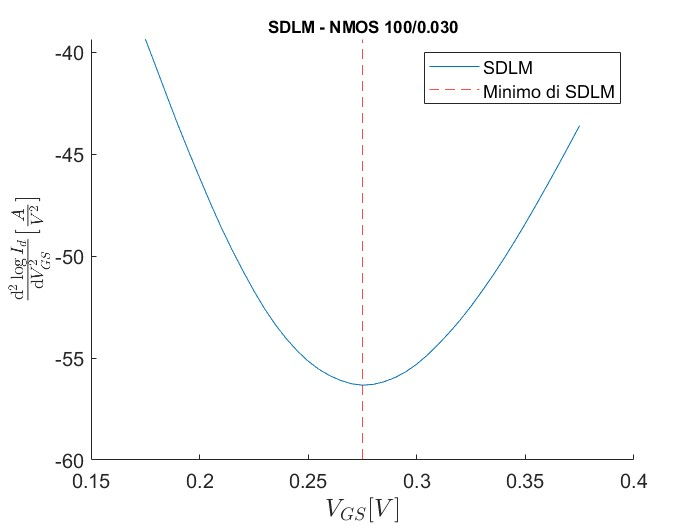
\includegraphics[width=0.49\textwidth]{SDLM-N4-100-30-NoFit}
  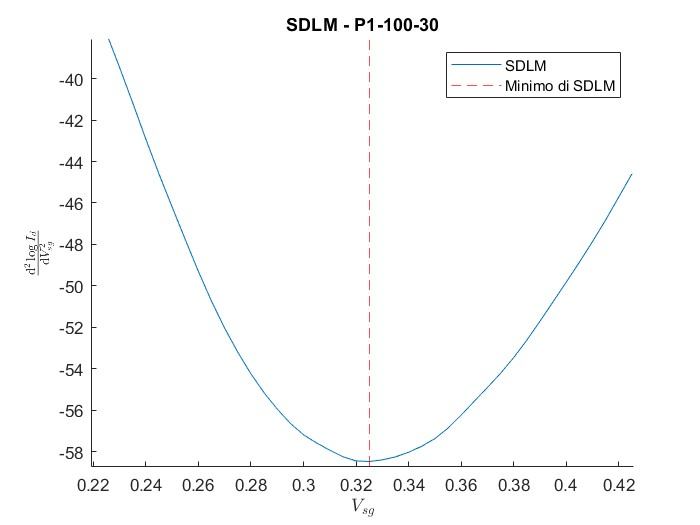
\includegraphics[width=0.49\textwidth]{SDLM-P1-100-30-NoFit}
  \caption{Esempio di \emph{SDLM} usato su un dispositivo NMOS e un dispositivo PMOS di dimensioni 100-30 a $V_{DS} = 900 mV$}
\end{figure}


% già detto prima
I due metodi appena esposti, però, sono molto sensibili ai picchi dovuti ad errori di misura e perciò sono difficilmente utlizzabili se prima non si rendono i grafici più puliti. Inoltre, la risoluzione del dispositivo di misura utilizzato e di $5 mV$, il che rende i valori ottenuti della $V_{th}$ molto approssimativi.
Per far fronte a questi due problemi, si è scelto di non tenere conto del minimo e del massimo direttamente ottenuti dalle derivate delle misure fatte, ma d'interpolare prima i punti dei grafici ottenuti con una funzione polinomiale e solo a questo punto di prendere in considerazione i picchi di minimo o di massimo. \\

\begin{figure}[H]
  \centering
  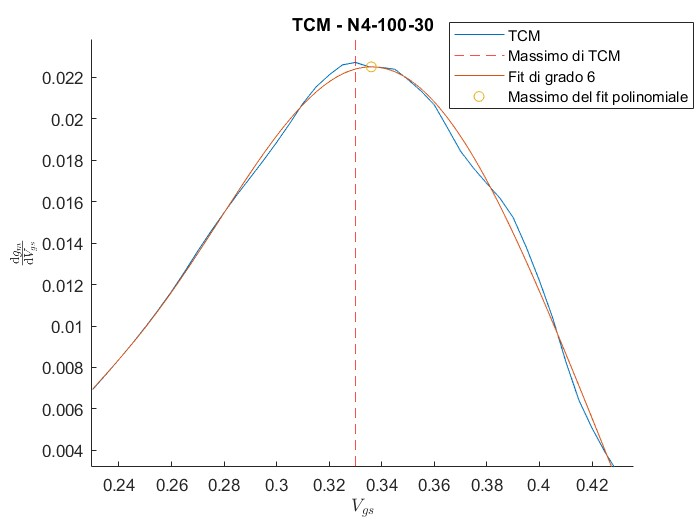
\includegraphics[width=0.49\textwidth]{TCM-N4-100-30}
  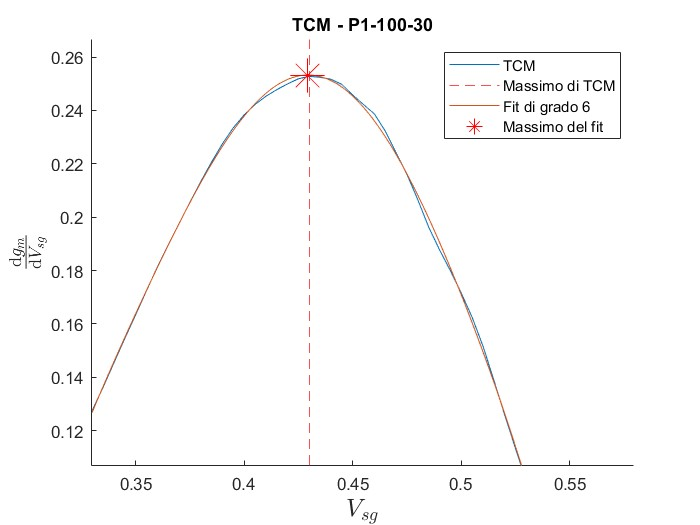
\includegraphics[width=0.49\textwidth]{TCM-P1-100-30}
  \caption{Esempio di \emph{TCM} con fit polinomiale usato su un dispositivo NMOS e un dispositivo PMOS di dimensioni 100-30 a $V_{DS} = 150 mV$}
  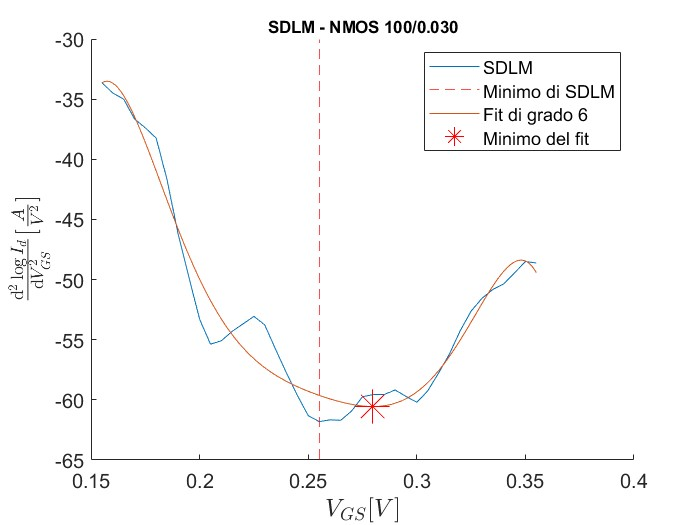
\includegraphics[width=0.49\textwidth]{SDLM-N4-100-30}
  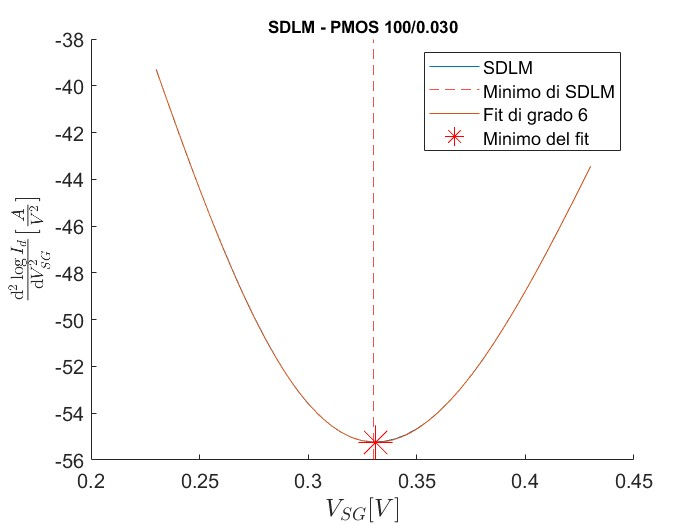
\includegraphics[width=0.49\textwidth]{SDLM-P1-100-30}
  \caption{Esempio di \emph{SDLM} con fit polinomiale usato su un dispositivo NMOS e un dispositivo PMOS di dimensioni 100-30 a $V_{DS} = 900 mV$}
\end{figure}

Per valutare l'accuratezza di questi due metodi si sono quindi calcolate le $V_{th}$ relative ai dispositivi di un PMOS, ottenendo i risultati seguenti:

\begin{table}[H]
  \renewcommand{\arraystretch}{1.3}
  \centering
  \begin{tabular}{m{4.4 cm} m{4.4 cm} m{4.4 cm}}
    \toprule
    Dispositivo & $V_{th} [mV]$ calcolata con TCM ($V_{SD} = 150 mV$) & $V_{th} [mV]$ calcolata con SDLM ($V_{SD} = 900 mV$) \\
    \midrule
    100 - 30    & 480.6                                               & 441.4                                                \\
    \hline
    100 - 60    & 469.3                                               & 411.6                                                \\
    \hline
    200 - 30    & 399.3                                               & 296.5                                                \\
    \hline
    200 - 60    & 453.5                                               & 404.9                                                \\
    \hline
    200 - 180   & 495.3                                               & 449.3                                                \\
    \hline
    600 - 30    & 385.9                                               & 289.7                                                \\
    \hline
    600 - 60    & 434.7                                               & 391.8                                                \\
    \hline
    600 - 180   & 480.6                                               & 441.4                                                \\
    \bottomrule
  \end{tabular}
  \caption{Valori di $V_{th}$ per i diversi dispositivi e con i metodi TCM e SDLM.}
  \label{tab:Iz*}
\end{table}

In generale i risultati sono abbastanza simili tra le due colonne, per cui si potrebbe prendere in considerazione uno di questi due metodi  per estrarre le tensioni di soglia e studiarne la degradazione.\\
È stato però notato un problema non indifferente: il valore della $V_{th}$ estratta dipende dal grado della funzione polinomiale che interpola i punti delle derivate usate per SDLM e TCM. La differenza dei valori estratti al variare del grado non è molto alta, si parla di pochi millivolt, perciò non influenza considerevolmente il valore della singola estrazione. Questa dipendenza, però, è problematica nel momento in cui si vuole studiare con precisione la degradazione delle prestazioni di un dispositivo all'aumentare dell'irraggiamento subito, in quanto piccoli spostamenti del valore di $V_{th}$ dovuti alla scelta arbitraria del grado della polinomiale può far variare eccessivamente le differenze delle misure tra un irraggiamento e l'altro, elemento inaccettabile se si considera che già le misure sono influenzate da errori casuali in fase di misura.\\
Come esempio si riporta il caso della \emph{SDLM} di un PMOS di dimensioni 600-30 con funzione polinomiale interpolatrice di grado 2, 4, 6 e 8. I valori della $V_{th}$ ottenuti sono:

\begin{table}
  \centering
  \begin{tabular}{c S[table-format=3.1]}
    \toprule
    {Grado della polinomiale} & {$V_{th} {[mV]}$} \\
    \midrule
    2                         & 296.0             \\
    \hline
    4                         & 291.4             \\
    \hline
    6                         & 289.7             \\
    \hline
    8                         & 298.1             \\
    \bottomrule
  \end{tabular}
  \caption{Valori di $V_{th}$ per diverse gradi di polinomiale.}
  \label{tab:valori_Vth}
\end{table}


\begin{figure}[H]
  \centering
  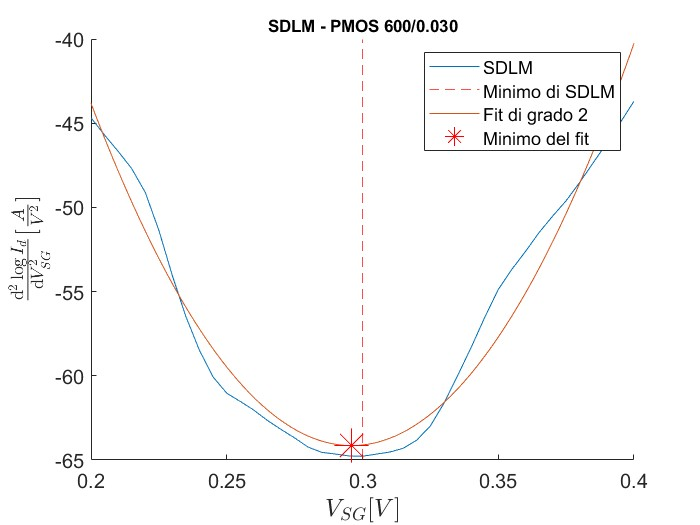
\includegraphics[width=0.49\textwidth]{SDLM-P1-600-30-grado2}
  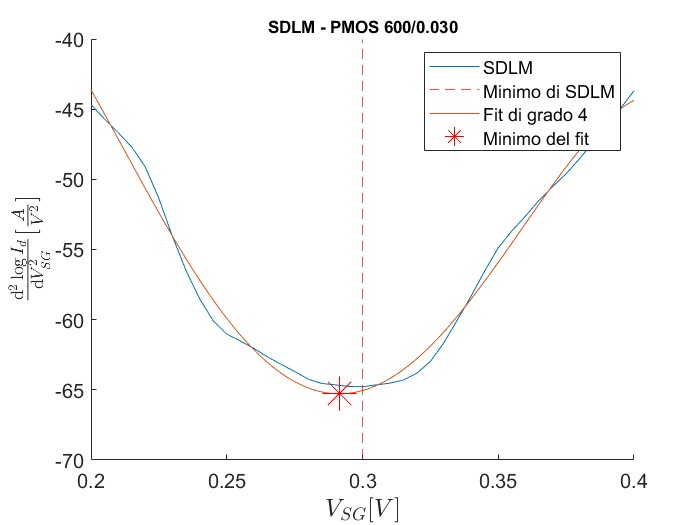
\includegraphics[width=0.49\textwidth]{SDLM-P1-600-30-grado4}
  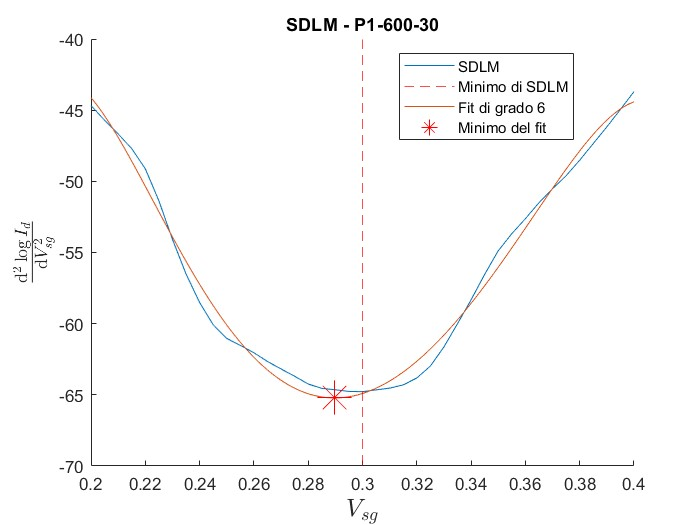
\includegraphics[width=0.49\textwidth]{SDLM-P1-600-30-grado6}
  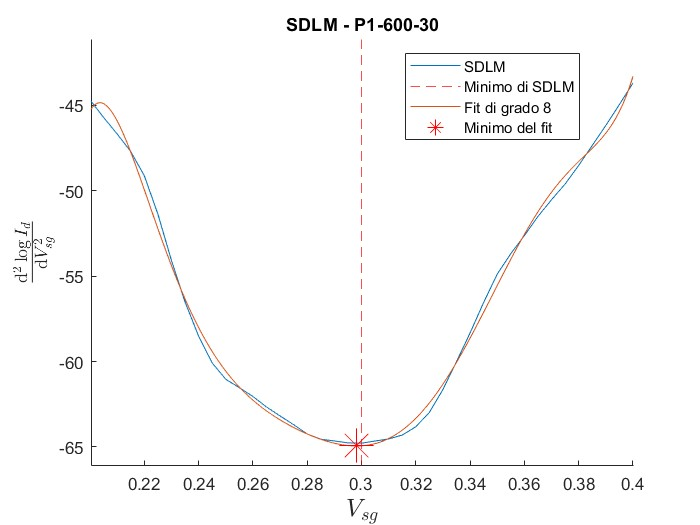
\includegraphics[width=0.49\textwidth]{SDLM-P1-600-30-grado8}
  \caption{Esempi di grafici di \emph{SDLM} su un PMOS di dimensioni 600-30 con fit polinomiale di diversi gradi}
\end{figure}



Per questo motivo si è valutato di utilizzare un terzo metodo: l'\emph{Extrapolation in the Linear Region method, ELR}, con il quale si ottiene la misura della $V_{th}$ attraverso l'analisi della caratteristica $I_D-V_{GS}$.  Tale grafico presenta un punto di flesso attorno al quale il grafico è linearizzabile. Tracciando il fit lineare nell'introno del punto di flesso si ottiene un retta che interseca l'asse delle ascisse, ovvero quello di $V_{GS}$, in un punto il cui valore corrisponde a quello della $V_{th}$.\\


\begin{figure}[h!]
  \centering
  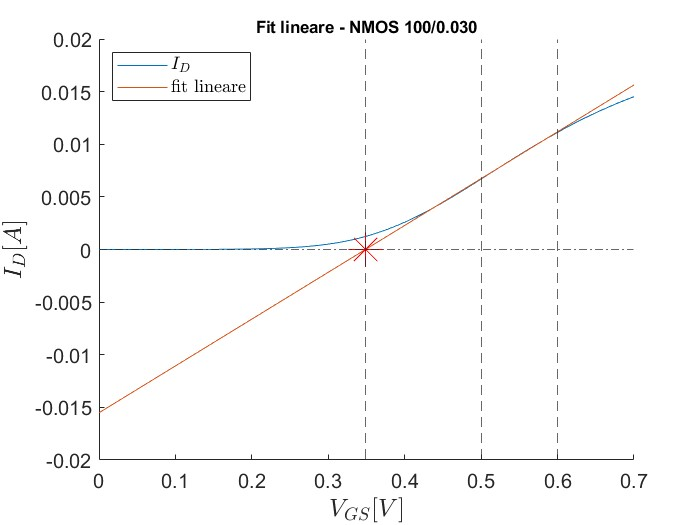
\includegraphics[width=0.49\textwidth]{LinearFit-N4-100-30}
  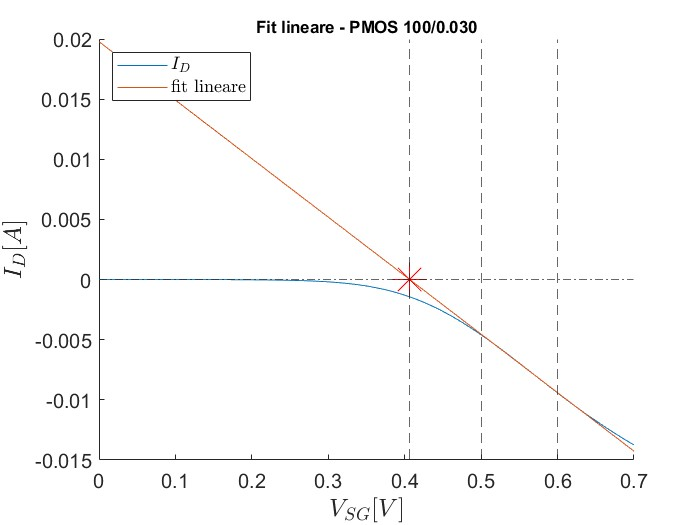
\includegraphics[width=0.49\textwidth]{LinearFit-P1-100-30}
  \caption{Fit lineare della caratteristica  $I_D$-$V_{GS}$ a $V_{DS}=150mV$ di un NMOS e di un PMOS di dimensioni 100-30 nell'intorno $[0,5V ; 0,6V]$ di $V_{GS}$}
\end{figure}

Di per sé, questo metodo è meno preciso di quelli esposti precedentemente, però è più affidabile nella misura delle differenze di $V_{th}$ man mano che i dispositivi vengono irraggiati. Problema con le resistenze parassite















\end{document}